% % äöüß
\chapter{Introduction}
\addcontentsline{lof}{chapter}{\thechapter\hspace*{1ex} Introduction}
%
The second half of the 20$^\text{th}$ century was characterized by the advance of semiconductor electronics that led to the invention of computers, affecting most parts of today's daily life.
Most commonly the semiconductor material silicon is used, being the second most abundant element in the Earth's crust and having already been used for fabrication of ordinary glass for centuries.
One of the key elements that enabled the breakthrough of semiconductor technology is doping, \ie the introduction of electron donating or accepting impurities that allow for controlling of the majority charge carriers. Doping enables the design of p-n-junctions, being the building block for most electronic devices, from transistors to light-emitting diodes and photovoltaic cells. Furthermore, it allows for adjusting the conductivity over orders of magnitude by increasing the charge carrier density and therefore tuning charge injection, extraction and transport properties.

Recently, semiconductors composed of chemically synthesized organic (\ie hydrocarbon-based) molecules increasingly gained attention, since organic dyes with delocalized $\pi$-systems have promising properties for optoelectronic devices.
The major drawback of organic semiconductors is their rather low charge carrier mobility, being several orders of magnitude below the values of typical conventional semiconductors. This is due to the weak interaction between adjacent organic molecules in a layer that leads to a slower charge-transfer between the molecules, compared to the almost unhindered band transport in a crystalline inorganic semiconductor formed by covalently bound atoms.
%
But, whereas a limited variety of conventional (inorganic) semiconductor materials is available, the toolbox of organic chemistry allows to design and synthesize molecules with desired properties.

The optoelectronic properties of organic semiconductors led to the development of organic light-emitting diodes (OLED) and organic photovoltaic cells (OPV), converting electricity to light and vice versa. The lower refractive index of organic semiconductors compared to conventional semiconductors allows for good light in- and outcoupling. In the last 15\,years, the development of both technologies was accompanied by an exponentially increasing number of publications over time that drove exponentially increasing record efficiencies, as shown in \figref{oled+opv-pub+eff}.
In contrast to conventional electronics, both types of devices, OLEDs and OPV, can in principle be fabricated on foils allowing for flexible lightweight devices and large device areas, which opens new areas of applications.
The main drawback is that device lifetime is limited by reactions with water and oxygen, requiring exceptionally good encapsulation.
Device thicknesses in the range of just hundred nanometers and low fabrication temperatures with typical substrate temperatures below \grad{100} lead to very low material and energy consumption and hence promise low production costs.

\begin{wrapfigure}[32]{r}[5mm]{62.8mm}% width aus grafic auslesen
\vspace*{-0.5cm}
% #1=lines #2=placement #3=overhang into margin # 4=width
{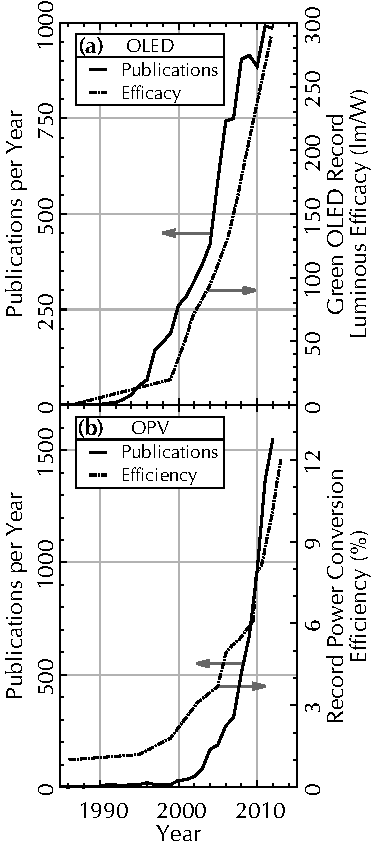
\includegraphics{plot/oled+opv-pub+eff}}
\caption
[OLED and OPV publications per year and laboratory ``hero'' performance]
{(a) OLED and (b) OPV publications per year and laboratory ``hero'' performance.\cite{OW,ISI}
}
\label{fig:oled+opv-pub+eff}
\end{wrapfigure}%
%
%
OLEDs are developed for lighting as well as for display applications.
OLED lighting competes with fluorescent lighting as well as inorganic light-emitting diode (LED) technology.
%
While LEDs are usually point light sources, OLEDs are natural area emitters of diffuse light and allow for new design options like transparent lighting panels. At the time of writing, first products are commercially available.
%
OLEDs for display applications have already proven their potential and successfully emerged into markets where they are competing with conventional liquid crystal display (LCD) technology. Key advantages of OLED displays are higher contrast, potentially low power consumption, smaller thickness and larger viewing angle, mostly enabled by the direct emission of light with the desired color instead of a combination of white backlight and color filters like in LCDs.

Organic semiconductor-based photovoltaics is a promising candidate for providing future electricity supply. Besides silicon-based photovoltaics, it seems to be the only non-concentrated technology with sufficient raw material available for a TW-scale production\cite{Feltrin2008}, required for a significant share of worldwide supply of sustainable electricity.
While for silicon-based photovoltaics the record efficiencies stagnated in recent years and only the production costs could be dramatically reduced, in the last 15 years exponentially increasing OPV record efficiencies have been reported, as shown in \figref{oled+opv-pub+eff}\,(b).
%
At the time of writing, a record power conversion efficiency of 12\,\%\cite{Heliatek12.0} 
is published which is below the record for polycrystalline silicon cells (20.4\,\%)\cite{SolarCellEff41} but already above the value for amorphous silicon (10.1\,\%)\cite{SolarCellEff41}.
In contrast to inorganic cells, the efficiency is stable between room temperature and elevated operating temperature and a better low-light performance is reported \cite{Riede2011,Heliatek12.0}.
%
The major drawback for polycrystalline silicon-based photovoltaic modules is the rather long energy payback time (\eg $\approx 2$ years when installed in Germany\cite{PV-Fakten201303}). Roll-to-roll processing of OPV modules on flexible substrates might allow for a high production throughput and hence, together with low material consumption and low fabrication temperatures, enable short energy payback time and low cost\cite{Anctil2012}.
Furthermore, the narrow absorption bands of organic semiconductors allow for fabrication of color-tunable semi-transparent cells as well as for efficiency-optimized tandem or triple cells\cite{Riede2011,Heliatek12.0}.

Two classes of organic semiconductors are typically distinguished: polymers and small molecules.
Polymers are large molecules consisting of repeating structural units and are typically deposited by wet chemical methods like coating or printing from solution. They show higher charge carrier mobilities than small molecules due to their intra-molecular transport, but chain length dispersity and solvent contamination hamper reproducibility.
Small molecules are compounds of rather low molar mass, often allowing for purification and deposition by thermal evaporation, typically in vacuum. Charge carrier mobilities are usually lower than in polymers and the initial cost for large scale production by vacuum deposition tends to be larger compared to solution processing of polymers. However, the thermal evaporation process allows for freely designable multilayer devices, which is hardly possible for polymers, due to the interaction of solvents with layers already deposited and the lack of orthogonal solvents.

Organic semiconductors can be doped by co-depositing electron donating or accepting atoms or molecules along with the host material. Doping of organic semiconductors has been shown to improve device performance significantly\cite{Walzer2007,LuessemRiedeLeo2013-PSS}, but contrary to conventional semiconductors, the underlying physics is far from being completely understood.
It is the aim of this thesis to contribute to the understanding of the fundamental physics of doping of organic semiconductors by studying the molecular doping in vacuum deposited layers of organic small molecules.

This thesis is structured into nine chapters. Following this introduction, chapter~\ref{chap:Theo} provides the theoretical background and reviews relevant literature for the studies presented in the subsequent chapters. In chapter~\ref{chap:Exp},
the experimental techniques as well as the developed setup are explained in detail. Furthermore, the investigated organic compounds are introduced and their key properties along a draft historical background are summarized.
The presentation of the results starts in chapter~\ref{chap:PaddleWheels} with investigations of the fullerene \CS n-doped by the two novel dopants \CrPd and \WPd of extremely low \IEs and which hence are reactive to air. The degradation induced by air-exposure of doped layers is studied and a regeneration treatment is presented.
In chapter~\ref{chap:AirStables}, \CS is n-doped by air-stable precursor compounds (\aob, \dmbi and \meodmbiI) that form the active dopant compound during deposition. This transformation is investigated more closely for the two novel DMBI derivatives.
Following the studies of n-doping, in chapter~\ref{chap:P-Doping} two amorphous hosts (\meo and \lili) are p-doped by two different dopants (\FS and \CSF) and the influence of the molecular energy levels on the doping is analyzed.
Afterwards, in chapter~\ref{chap:P5} the model system of the polycrystalline host \pen p-doped by the similar-sized dopant \FV is investigated and the data are compared to theoretical predictions for this combination.
Finally, in chapter~\ref{chap:Rech} a model is developed that allows to derive lower limits for the charge carrier mobility, the \nLong as well as the \DopEffLong from conductivity data and furthermore allows to narrow down the energetic position of the \EtLong level when combined with Seebeck data.
Concluding, the findings of this thesis are summarized in chapter~\ref{chap:summary} and directions for future studies are outlined.

